
\chapter{Introduction}
\label{cha:intro}

In this intermediate report we describe the activities to formally verify
the correctness of parts of the software developed in the OpenETCS project.

While major parts of the functionality of {Subset 026} are modelled in 
higher-level languages, there is also a substantial part of \emph{supporting} software
that is developed in the~\isoc programming language.

In this document we report about results on the verification of that \isoc~code.
In particular, we report on the use of static analysis methods (including formal methods)
on \isoc~code that has been developed by the project partner Siemens.

\begin{figure}[hbt]
\begin{center}
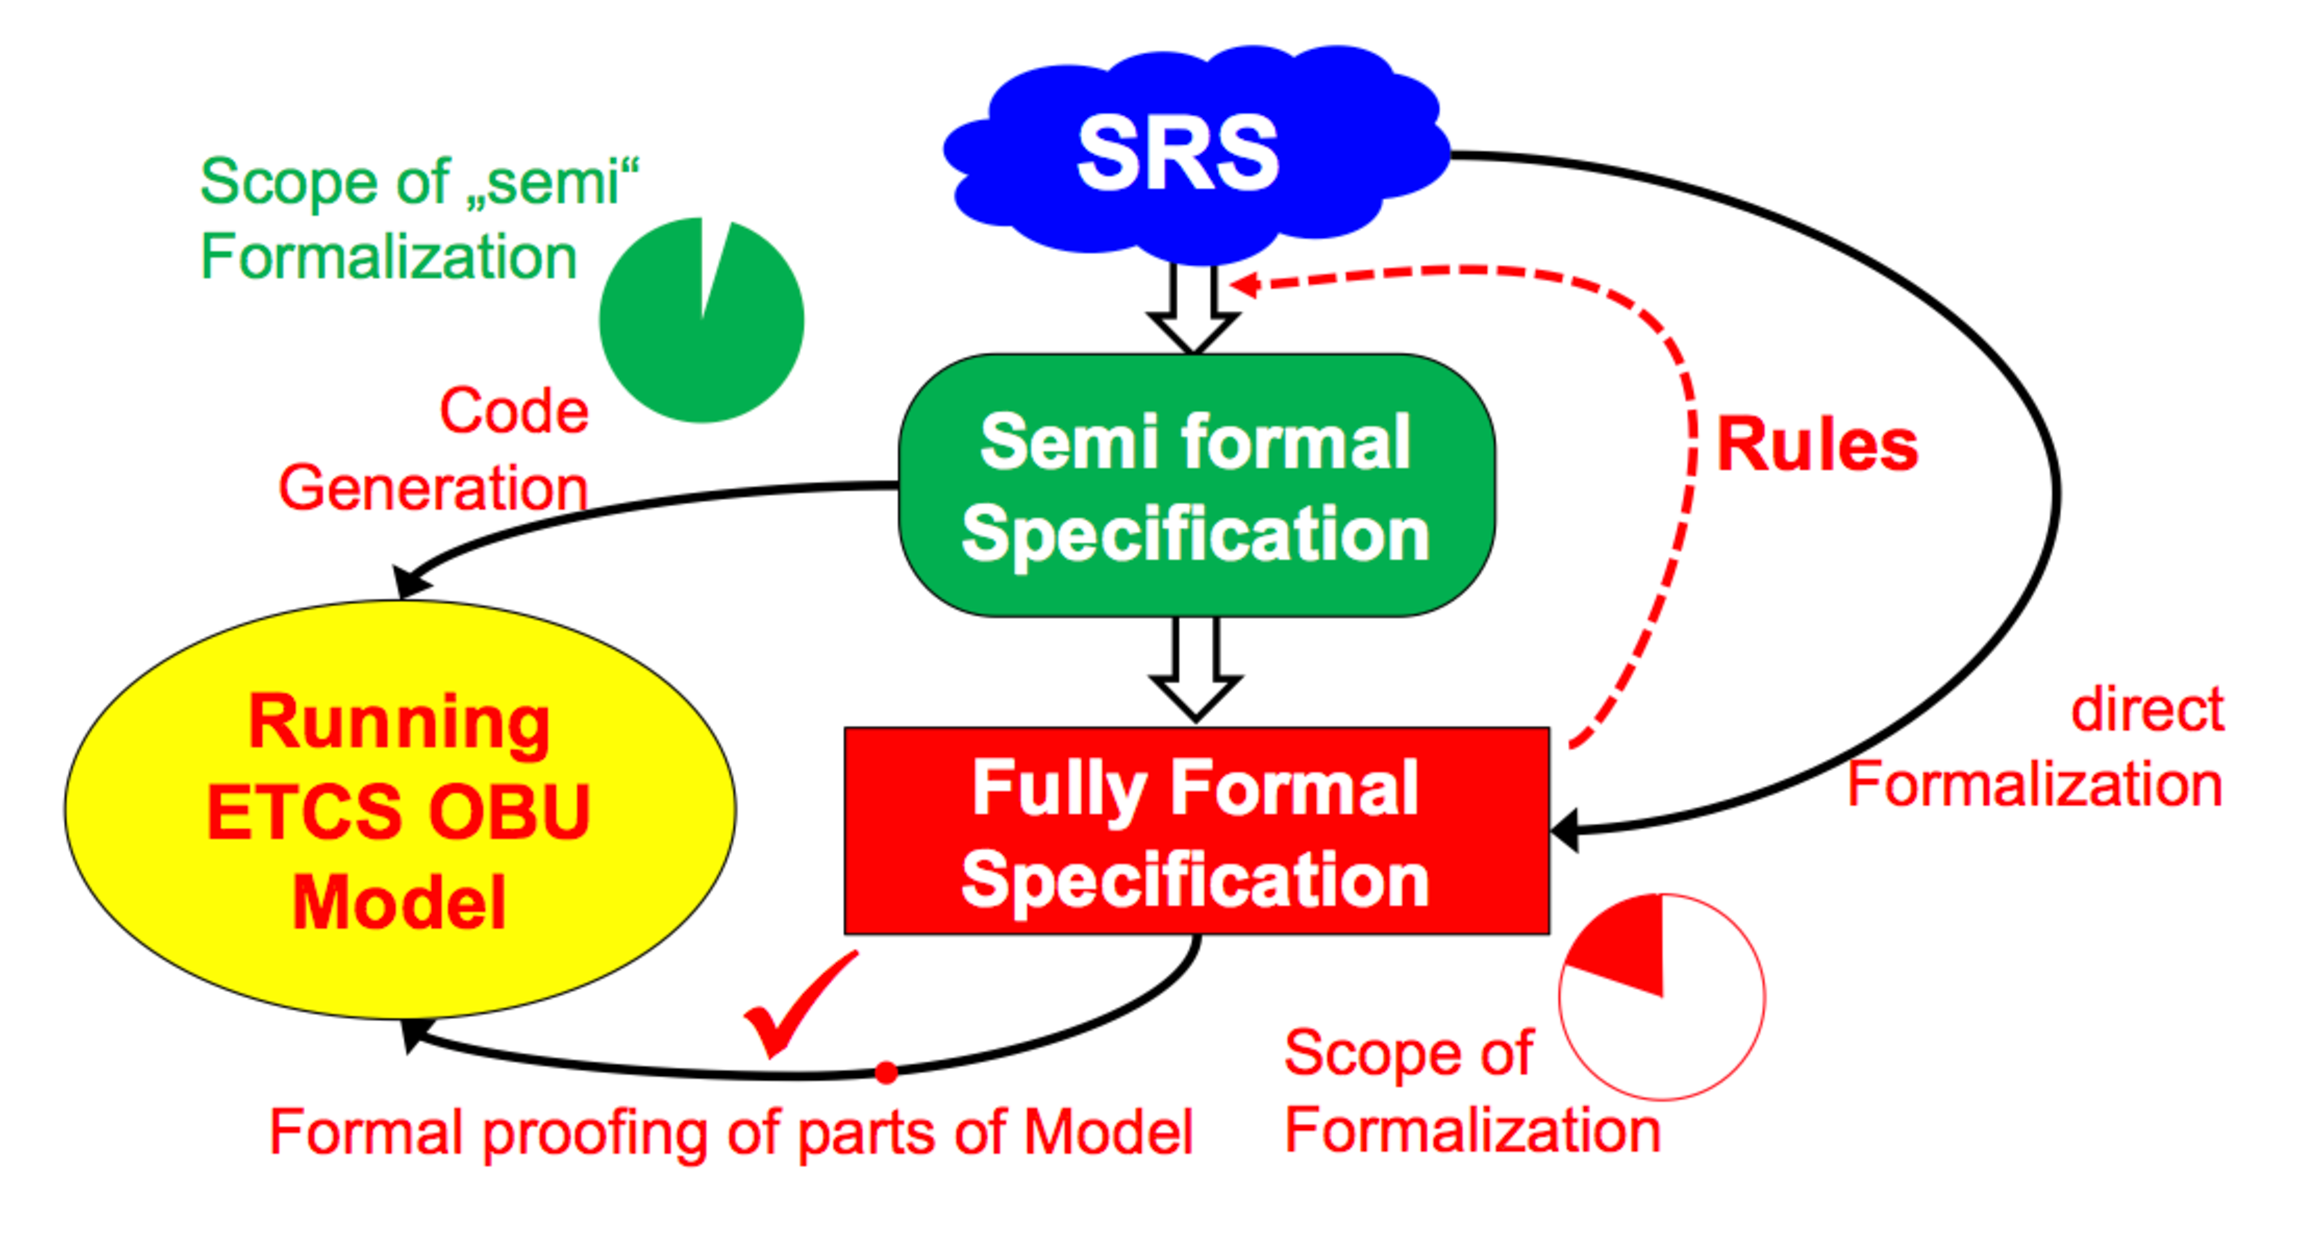
\includegraphics[width=0.95\textwidth]{figures/scope-of-formalization.pdf}
\caption{\label{fig:scope-of-formalization} Scope of formal methods with in OpenETCS}
\end{center}
\end{figure}

Figure~\ref{fig:scope-of-formalization} outlines the roles of formal methods
within the OpenETCS project.
What this figure shall convey is that even a subsystem such as described by
\emph{Subset 026} of the ETCS specification
is usually too complex to be completely formally specified.
Therefore, \emph{semi-formal modelling techniques} and \emph{tests} and 
\emph{simulations} play a crucial role to verify that the implementation
satisfies its specification.
However, for clearly defined modules and select system properties, formal methods
can well be applied to establish the correctness of an implementation.

Figure~\ref{fig:scope-of-code-verification} shows slightly more detailed
the OpenETCS software.
The report at hand is limited to the parts encapsulated by \isoc software encapsulated 
in a \dbox{dashed box}.

\clearpage

\begin{figure}[hbt]
\begin{center}
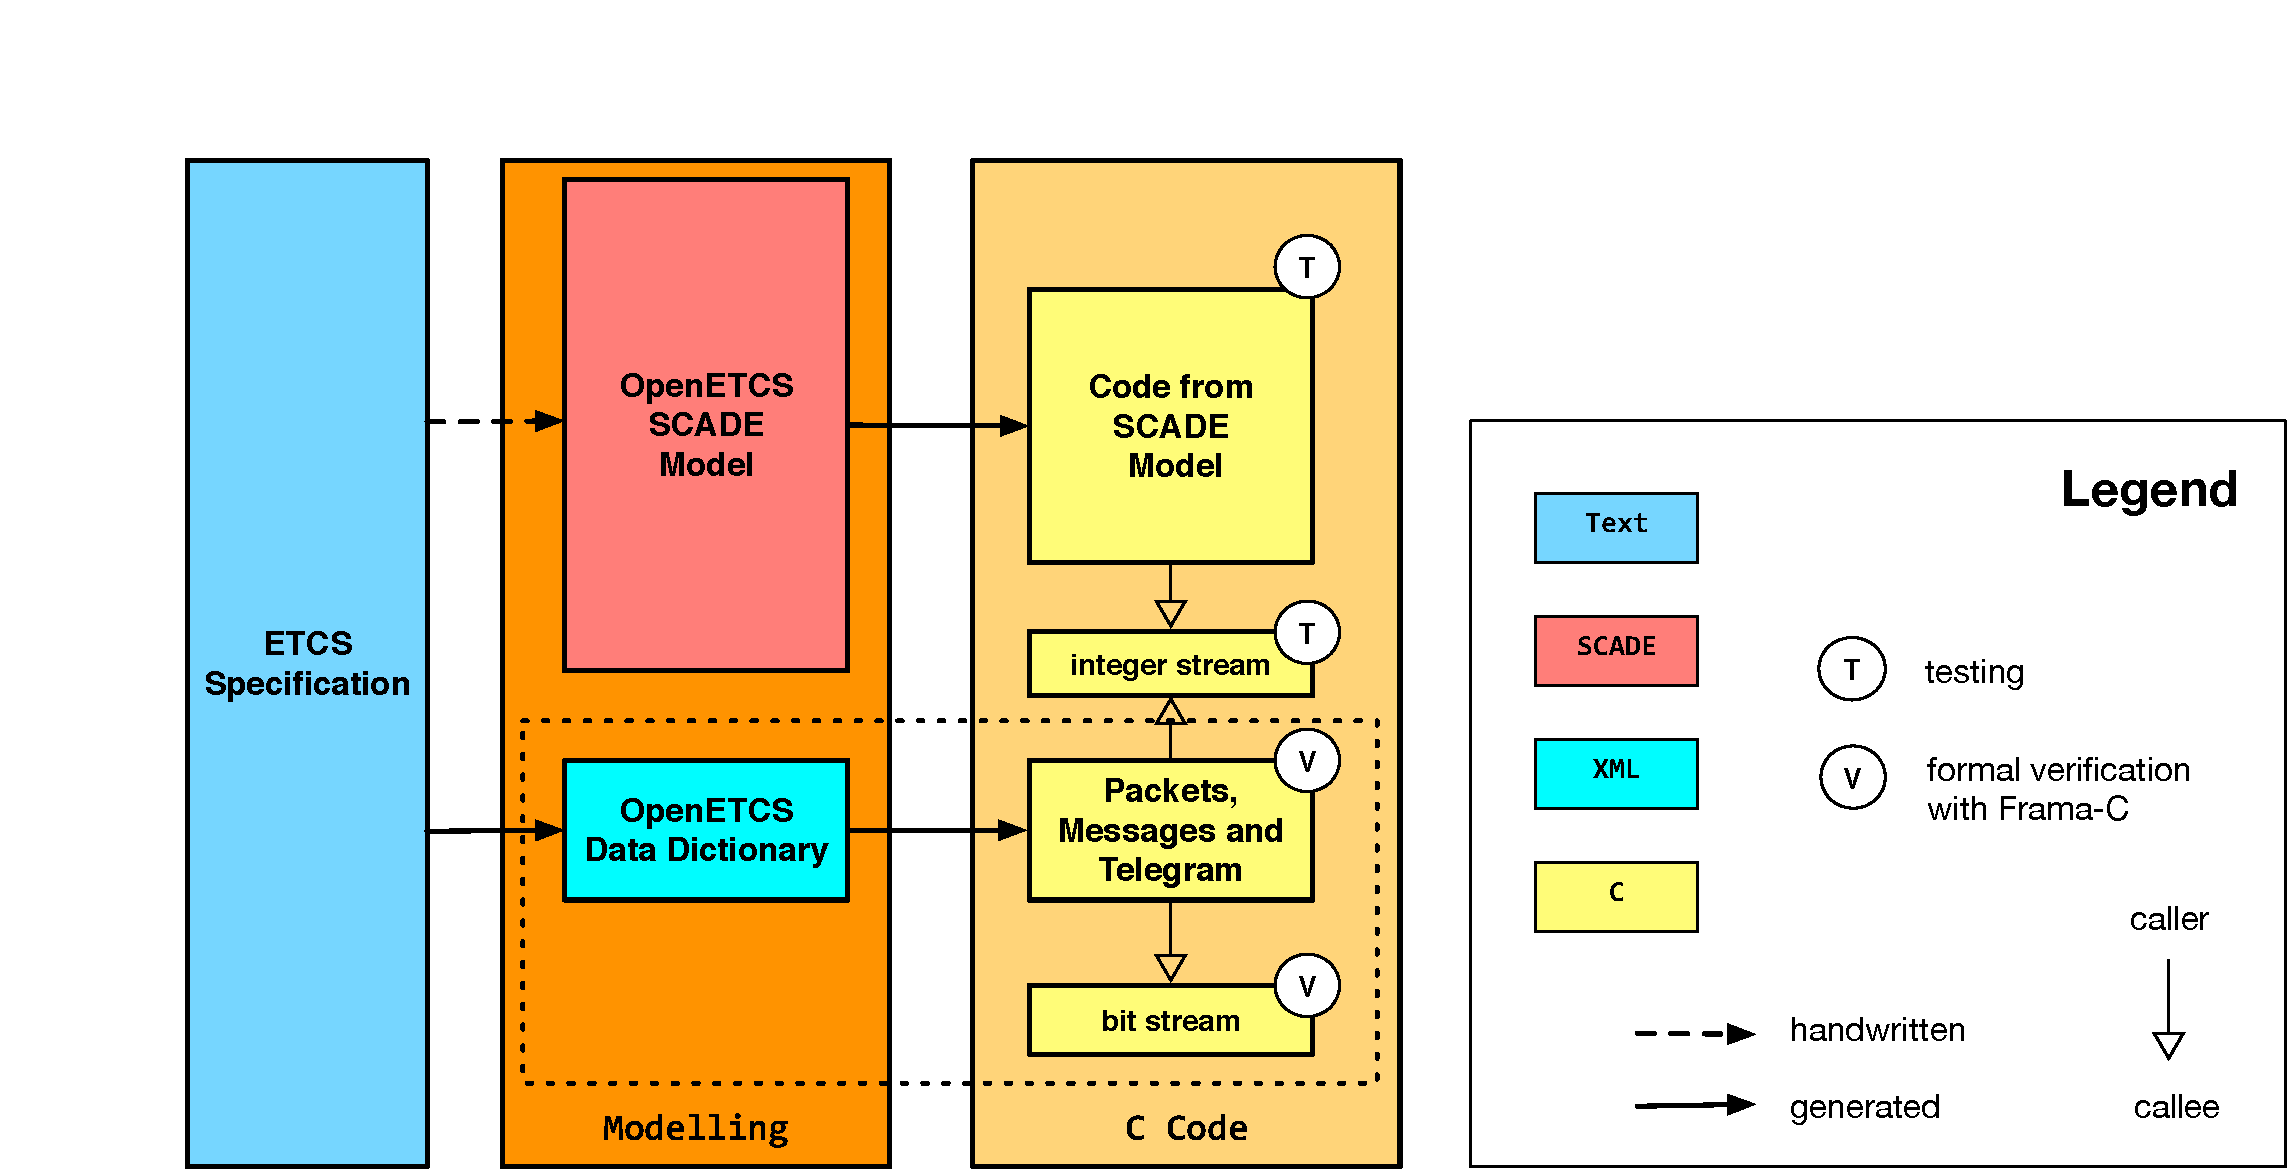
\includegraphics[width=0.95\textheight,angle=90]{figures/OpenETCS-Stack.pdf}
\caption{\label{fig:scope-of-code-verification} Scope of code verification}
\end{center}
\end{figure}

\FloatBarrier

\section{Software layers}

Figure~\ref{fig:software-layers} shows the layer structure of the OpenETCS \isoc~code.
The OpenETCS decoder\slash encoder is a collection of data structures and associated functions
for reading and writing ETCS packets from\slash to a bit stream.

\begin{figure}[hbt]
\begin{center}
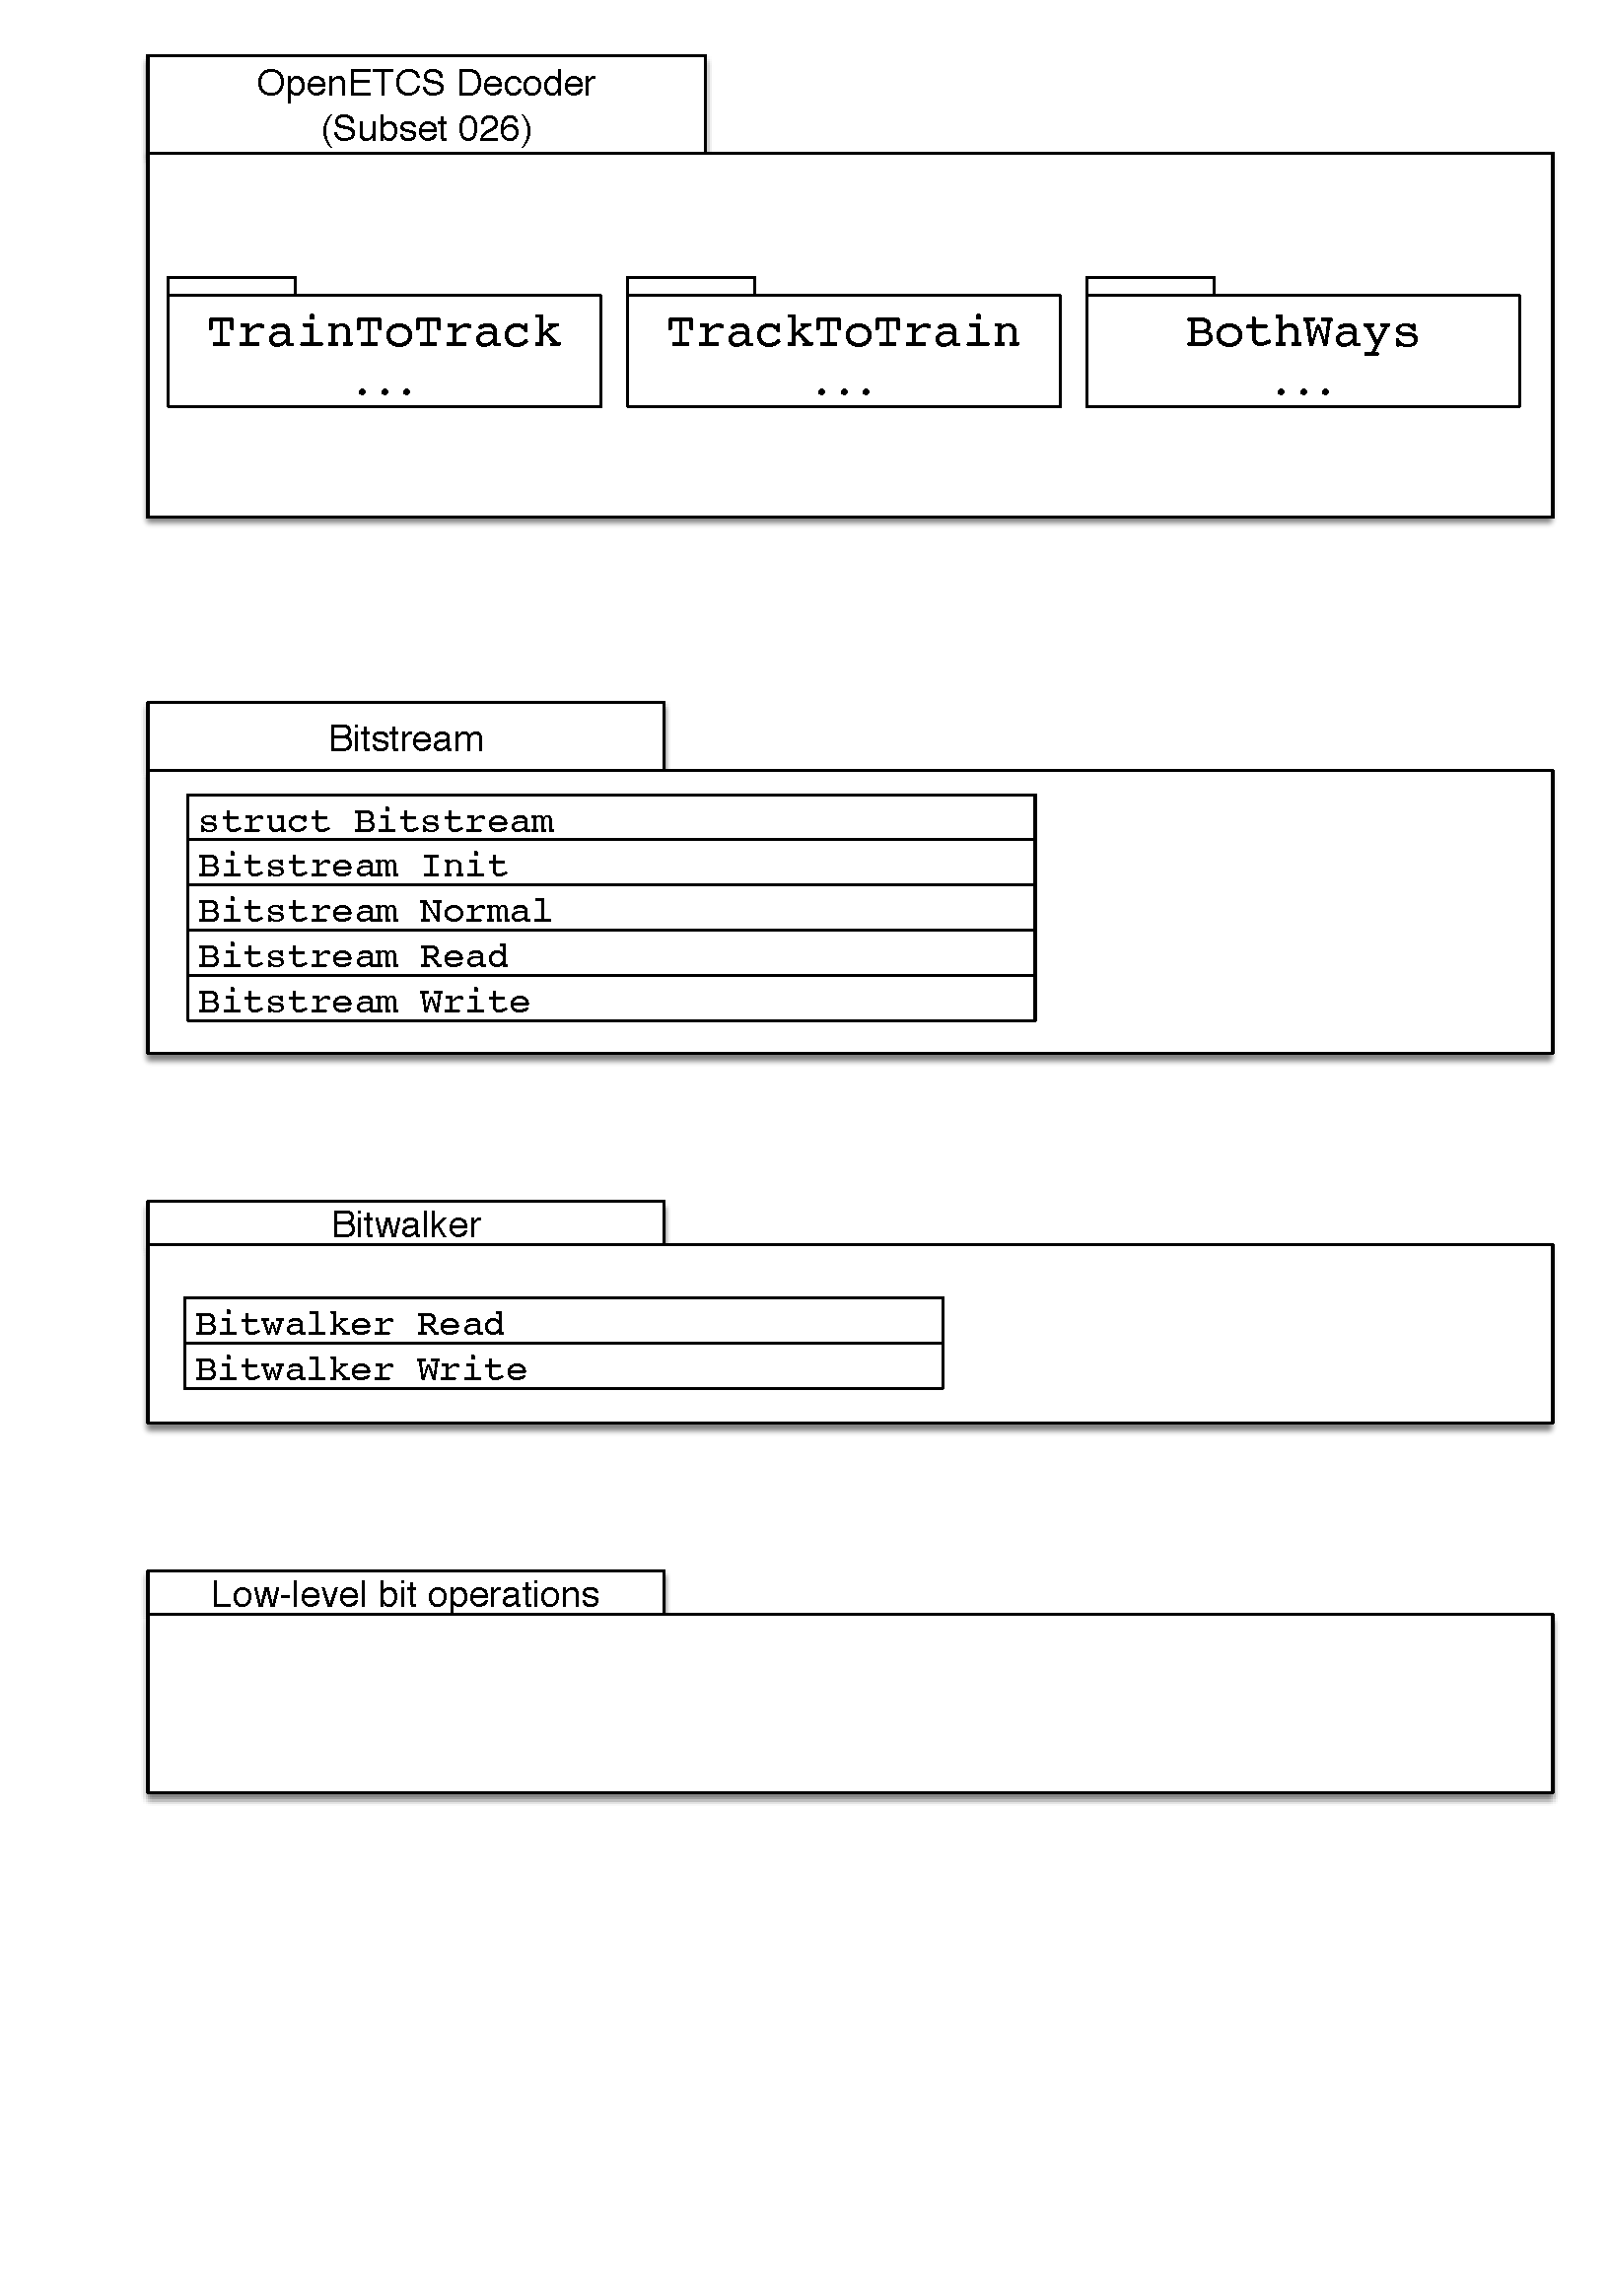
\includegraphics[width=1.0\textwidth]{figures/software-layers.pdf}
\caption{\label{fig:software-layers} Software layers of the OpenETCS \isoc~code}
\end{center}
\end{figure}

\FloatBarrier

In order to fulfill their task the decoder and encoder function rely on an
implementation of bit streams in \isoc.
The \inl{Bitstream} package in turn is built on top of the so-called \emph{bitwalker} layer.
In order to accomplish the task of formal verification of these layers 
we also provided several functions that read and write individual bits for basic \isoc~types.

The main achievement that we present in this report are the results
on the formal specification and formal specification of the various software layers 
in Figure~\ref{fig:software-layers}.

This report is result of the joint work of many OpenETCS partners, notably:

\begin{itemize}
\item CEA LIST
\item DLR
\item Fraunhofer FOKUS
\item Siemens
\item SQS
\end{itemize}

The formal analyses contribute to the ultimate verification goals,
which are the following:

\begin{enumerate}
\item provide evidence that both the generated and a handwritten \isoc~code satisfies 
      accepted quality standards
\item develop a formal specification for Subset~026 functionality
\item verify with \framacwp that the software satisfies its formal specification
\item show that the software does not raise runtime errors
\end{enumerate}

The European standard for railway software~\cite[\S~7.3.4.19]{en50128-2011} mandates that 
the specification of software interfaces shall address various properties.
Table~\ref{tbl:software-interfaces-en50128} list these properties and also indicates
to what extend \framac can be used to formally express them.


\begin{table}[hbt]
\begin{center}
\begin{tabular}{|p{8cm}|c|}
\hline
\textbf{Property} & \textbf{Specification through \framac} \\
\hline
pre and post conditions & yes \\
\hline
definition and description of all boundary values for all specified data & yes \\
\hline
behaviour when the boundary value is exceeded & yes \\
\hline
behaviour when the value is at the boundary & yes \\
\hline
time-critical input and output data & no \\
\hline
allocated memory for the interface buffers and the mechanisms to detect that the memory cannot be allocated or all buffers are full, where applicable & yes \\
\hline
existence of synchronization mechanisms between functions & partially \\
\hline
\end{tabular}
\end{center}
\caption{\label{tbl:software-interfaces-en50128} Properties to be addressed by interface specification according to EN~50128}
\end{table}

We see from this table that \framac\footnote{%
	Or to be more precise ``\acsl'' (ANSI\slash ISO-C Specification Language) which
	is the specification language of \framac.
}
is a well-justified choice for the specification of railway software.

\section{Structure of this document}

We represent the \isoc~code and related specifications in a top-down approach.
Thus, we start on the level of OpenETCS data packets and explain from there
the lower software levels.

\begin{itemize}
\item
Chapter~\ref{cha:frama-c} gives a short overview on the \framacwp tool
that plays a central role in the verification of OpenETCS \isoc~code.
Here we also try to rectify some misunderstandings about formal verification
that we have encountered in our work.

\item
Chapter~\ref{cha:packets} presents the formal specification of OpenETCS
packets in \acsl (the specification language of \framac).
For the sake of an easier understanding we start with the specification of
a concrete packet (\adhesion in Section~\ref{sec:adhesionfactor})
and explain from there how the other specifications look like.

\item
The OpenETCS packets are written to and read from bit streams which is represented
by the type \inl{Bitstream} and its associated functions.
Chapter~\ref{cha:bitstream} provides the definition and formal specification
of \inl{Bitstream} operations.

The implementation of \inl{Bitstream} itself relies on lower level bit operations.
The formal specification of these operations are presented in Chapter~\ref{cha:low-level bitstream}.

\item 
Chapter~\ref{cha:formal-verification} lists results of the formal verification with \framacwp.

\item
In Chapter~\ref{cha:conclusions}, we draw conclusions from this work
and outline the next steps in our verification efforts.
\end{itemize}

